\chapter{Einleitung}

Eine oft genutzte technische Anwendung der Sportmedizin ist die Leistungsdiagnostik zur Bestimmung individueller, zielorientierter Trainingsbereiche. Hierzu gibt es zwei von einander unabhängige Verfahren: die Betrachtung der Laktatkinetik durch Blutentnahme und die Spiroergometrie (aus lat. \textsl{spirare}: atmen, griech. \textsl{ergo}: Arbeit) mit Analyse von respiratorischen Daten während steigender körperlicher Belastung~\cite{Westhoff.2012} . Der große Vorteil der Spiroergometrie besteht darin, dass sie anders als die Laktatdiagnostik nicht-invasiv ist. Früher wurde sie allerdings nur in speziellen Sport- oder Funktionslaboren bei ärztlichem Fachpersonal angeboten, war darüber hinaus sehr kostenintensiv und deshalb nur für hoch ambitionierte Leistungssportler eine gute Investition. Jedoch ist besonders der Markt für den Breitensport in den letzten Jahren stetig im Wachstum und Statistiken zeigen einen deutlichen Aufwärtstrend der Fitness-Wirtschaft. Zwischen 2014 und 2017 stieg die Gesamtanzahl an Mitgliedern in deutschen Fitnessstudios und Gesundheitszentren um 14,4 \% von 9,08 Mio. auf 10,61 Mio.~\cite{DSSV.2018}. In einer Umfrage des Arbeitgeberverbandes deutscher Fitness- und Gesundheits-Anlagen (DSSV e.V.) positionierten sich 2017 rund 44 \% aller deutschen Fitnessanlagenbetreiber im Sektor Gesundheit und Prävention. Dieser stellt für den Hamburger Medizintechnik-Hersteller \textsl{cardioscan GmbH} den größten Abnehmer dar. Die Firma bietet für eine Vielzahl an diagnostischen Bereichen MPG-zertifizierte Systemlösungen in Form von Software oder Hardware, die bereits bei vielen internationalen Kunden im Einsatz sind. Die meistverkauften Analysesysteme sind das Ruhe-EKG, die Bioimpedanzanalyse sowie das Stoffwechsel-Messgerät \textsl{metabolicscan}, das cardioscan im Jahre 2017 entwickelt hat. In Verbindung mit der dazugehörigen \textsl{\ac{CCPS}} und unterschiedlichen Fahrradergometern ist der metabolicscan auch für die Spiroergometrie geeignet. Die \acs{CCPS} enthält sowohl die Steueroberfläche, als auch einen Auswertungsalgorithmus zur automatischen Bestimmung der Trainingsbereiche. Jener ist derzeitig allerdings recht sensitiv für Abweichungen und Fehler bei bestimmten Personengruppen und soll zukünftig dahingehend optimiert werden, dass die Messungen auch für jene Personen valide Ergebnisse liefern. Deshalb sollen neue Algorithmen zur Bestimmung der beiden sogenannten ventilatorischen Schwellen evaluiert werden, anhand derer die Trainingsbereiche für eine Person zuverlässiger definiert werden können.

\section{Physiologische Grundlagen}

Grundsätzlich werden heutzutage in der Spiroergometrie zwei von Prof. Karlman Wasserman geprägte Schwellen identifiziert, anhand derer die Trainingsbereiche Regeneration/Kompensation, extensive sowie intensive Grundlagenausdauer, Entwicklung und Leistung bestimmt werden. Dieses ventilatorische Schwellenkonzept beruft sich auf die nachweisliche physiologische Reaktion des Metabolismus auf erhöhte Belastung und hängt direkt mit der momentanen Energiebereitstellung des Körpers zusammen~\cite{Westhoff.2012}. Um diese Zusammenhänge nachzuvollziehen, wird zunächst auf die Mechanismen der Energiegewinnung eingegangen.

\subsection{Innere \& äußere Atmung}

\begin{figure}[H]
	\centering
	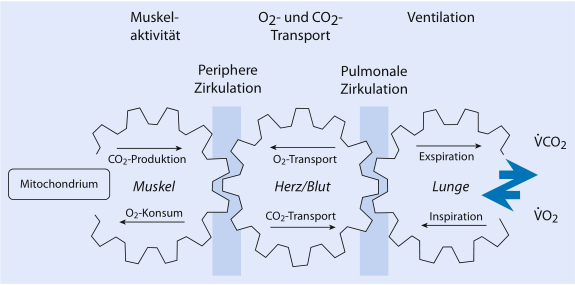
\includegraphics[scale=0.65]{Bilder/zahnraeder.png}
	\caption[3-Zahnräder-Modell mit physiologischen Interaktionen im Gasaustausch]{3-Zahnräder-Modell nach K. Wasserman mit den physiologischen Interaktionen im Gasaustausch~\cite{Loellgen.2010}}
	\label{pic:pic1}
\end{figure}

Ausgangspunkt der betrachteten physiologischen Prozesse ist die Atmungsventilation - also der Gasaustausch zwischen Umgebung, Lunge, Blut und Muskelzelle, wie in Abb. \ref{pic:pic1} veranschaulicht. Man kann prinzipiell zwischen "`innerer"' und "`äußerer"' Atmung bzw. peripherer und pulmonaler Zirkulation differenzieren. Die innere Atmung bezieht sich auf den molekularen Gasaustausch in den Mitochondrien. Die äußere Atmung betrifft den Transfer zwischen Blut und Lunge. Wesentlich sind hierbei die zwei in der Atemluft enthaltenen Fraktionen \ac{CO2} und \ac{O2}.
%
\begin{equation}
RQ = \frac{\dot{V}(CO_2)}{\dot{V}(O_2)}
\label{eq:formel1}
\end{equation}
%
Das Verhältnis von \ac{VCO2} zu \ac{VO2}, der Respiratorische Quotient (\acs{RQ}), muss normalerweise getrennt für die innere und äußere Atmung betrachtet werden. Bei gesunden Menschen bzw. bei idealer Zirkulation ohne Einschränkungen auf der Strecke des Gastransfers herrscht jedoch ein Gleichgewicht ("`Steady State"')~\cite{Kroidl.2015} und das 3-Zahnräder-Modell nach Wasserman (siehe Abb. \ref{pic:pic1}) funktioniert einwandfrei. Da kardiopulmonale Defizite in der Sportmedizin ein Ausschlusskriterium für eine Spiroergometrie darstellen, wird in dieser Arbeit generell von einem Steady State ausgegangen. Der RQ wird bei der Ruhestoffwechselanalyse gemessen und deutet an, aus welchen Makronährstoffen der Körper momentan Energie bezieht. Werden ausschließlich Fette metabolisiert, liegt er bei ca. 0,7. Dies ist in absoluter körperlicher Ruhe der Fall. Liefern Kohlenhydrate die gesamte Energie, nimmt er den Wert 1 an~\cite{Kroidl.2015}. Eine steigende Kohlenhydratverbrennung wird durch zunehmende Aktivität initiiert. Darauf fußt auch der aktuelle Software-Algorithmus von cardioscan. Die damit verbundene Problematik wird im Folgenden erläutert und diskutiert.

\subsection{Energiebereitstellung des Körpers}

\subsubsection{Primäre Energiebereitstellung}

Die Bewegung des menschlichen Körpers wird durch mechanische Kontraktionen der Skelettmuskulatur möglich. Hierfür dient die hydrolytische Spaltung des körpereigenen "`Brennstoffs"' \ac{ATP} als Energiequelle:
%
\begin{equation}
ATP + H_2O \rightarrow ADP + P_i + H^+
\label{eq:formel2}
\end{equation}
%
Mit der durchschnittlichen ATP-Konzentration im Muskel von \SIrange{5}{7}{\milli\mole\per\kg} lassen sich nur wenige Kontraktionen durchführen bzw. ein bis zwei Sekunden starke körperliche Arbeit verüben~\cite{DeMarees.1981}. Für längere Aktivität muss also stetig ATP resynthetisiert werden. Dies geschieht vorerst durch die anaerobe Reaktion von \ac{ADP} und \ac{CrP}~\cite{Heck.2006}. 

\begin{equation}
ADP + CrP + H^+ \leftrightarrow ATP + Cr
\label{eq:formel3}
\end{equation}

Kreatinphosphat kann mit einem Muskelgehalt von \SIrange{15}{20}{\milli\mole\per\kg} für ca. fünf bis sechs Sekunden körperlicher Last Energie liefern. Dementsprechend genügt diese Energiegewinnung nur für kurze Belastungsphasen. Mit weiterer andauernder und inkrementierter Belastung nimmt jedoch die CrP-Konzentration sehr steil ab und der Organismus greift auf sekundäre Energiequellen zurück.

\subsubsection{Sekundäre Energiebereitstellung}

Die sekundäre Energiegewinnung kann in die aerobe sowie anaerob-laktazide ATP-Resynthese differenziert werden~\cite{Kroidl.2015}. Durch zunehmende Belastung werden mehr zusätzliche Muskelfasern rekrutiert, welche die Energie schnell benötigen und aus Glukose beziehen. Die aerobe Glykolyse setzt zuerst ein, da sie mit insgesamt ca. \SI{36}{\mole} ATP pro Glukose-Molekül sehr effektiv ist~\cite{Kroidl.2015}. Der gesamte Prozess erfolgt enzymatisch in mehreren Teilschritten und endet mit dem Anion Pyruvat~\cite{Heck.2006}. Ist genügend Sauerstoff in den Mitochondrien vorhanden, kann das Pyruvat direkt in den Citratzyklus zur ATP-Resynthese überführt werden~\cite{Rassow.2008}. Bei zunehmender Belastung und damit auch erhöhtem \acs{O2}-Verbrauch kommt mit der Zeit die oxidative Kapazität zum Erliegen und das Redox-Coenzym \acs{NADH} reichert sich in unoxidierter Form an. Für die Glykolyse wird es allerdings als oxidiertes Substrat benötigt. Damit diese fortlaufen kann, hilft sich der Organismus selbst, indem er das Pyruvat durch das Enzym \ac{LDH} zu \ac{HLa}, bzw. deren Salz \ac{La-} reduziert~\cite{Rassow.2008} und die anaerob-laktazide Glykolyse aktiviert. Durch die dabei stattfindende Reoxidation des \acs{NADH}/\acs{H+} kann die Glykolyse, deren Rate bei zunehmender Muskelarbeit gesteigert werden muss, fortwähren~\cite{Heck.2006}. Das Laktat dient zu Beginn dieser Umstellung auch als Substrat für die Rückreaktion und akkumuliert zunächst in die Skelettmuskelfasern und anschließend im Herzmuskel~\cite{Klinke.2003}. Durch zunehmende Belastung steigen die \acs{H+}- sowie \acs{La-}-Konzentrationen weiter an und der Blut-pH-Wert sinkt. Dieser oftmals als "`Übersäuerung"' bezeichnete Zustand wird auch metabolische Azidose (aus lat. \textsl{acidum}: Säure) genannt~\cite{Boening.2008}. Hierzu kann die Nettoreaktionsgleichung der anaerob-laktaziden Glykolyse betrachtet werden:

\begin{equation}
Glukose \rightarrow 2 HLa \rightarrow 2 H^+ + 2 La^-
\label{eq:formel4}
\end{equation}

Infolgedessen wird das \acl{HCO3-}-Puffersystem des Körpers zur Aufrechterhaltung des natürlichen Säure-Base-Haushalts, dessen Reaktion Formel~\eqref{eq:formel5} darstellt, aktiv \cite{Kroidl.2015}.

\begin{equation}
NaHCO_3^- + H^+ La^- \rightleftharpoons CO_2 + NaLa H_2O
\label{eq:formel5}
\end{equation}

Das zusätzlich während dieser Prozesse entstehende \acs{CO2} muss nun mit dem \acs{CO2} aus der Energiebereitstellung über die Lunge eliminiert werden. Durch diese "`ventilatorische Kompensation"' kommt es zu einem messbaren Anstieg an exspiriertem \acs{CO2} im Verhältnis zum inspirierten \acs{O2}~\cite{Boening.2008}. Diese nachweisliche \ac{CO2}-Elimination gewährleistet letztlich die ventilatorische Schwellenbestimmung.\\

\section{Spiroergometrie}

\subsection{Ventilatorische Schwellen}

Somit kann die Energiebereitstellung eines Menschen grob in die Phasen aerob, aerob-anaerob und anaerob gegliedert werden~\cite{Antonutto.1995}. Die realen Zustände sind aber bei jedem Menschen sehr individuell und vermischt~\cite{Moosburger.1995}. Abhängig vom Gesundheits- oder Trainingszustand eines Menschen kann auch eine teilweise anaerobe Energiebereitstellung in Ruhe oder aber eine überwiegend aerobe bei hoher Belastung vorliegen~\cite{Skinner.1980}. Um individuell Trainingsbereiche definieren zu können, müssen diese Übergänge also zuerst bestimmt werden. Sie wurden einst als aerobe und anaerobe Schwellen deklariert~\cite{Wasserman.1973}. Da in Publikationen aus der Vergangenheit unterschiedliche Titel für die gleichen Schwellen auftauchten, wurden inzwischen mit der 1. und 2. Ventilatorischen Schwelle - abgekürzt als \acs{VT1} und \acs{VT2} - einheitliche Fachtermini festgelegt, die weitestgehend Verwendung finden~\cite{Westhoff.2012}.
\begin{table}[H]
	\centering
	\caption[Pathophysiologische Veränderungen an VT1 und VT2]{Pathophysiologische Veränderungen an VT1 und VT2~\cite{Westhoff.2012}}
	\medskip
	\begin{tabularx}{\textwidth}{X X}
		\toprule
		\textbf{VT1} & \textbf{VT2} \\
		\midrule
		\midrule
		Laktatanstieg mit Laktatpufferung zu Beginn des aerob-anaeroben Übergangs & Überschreiten des Max. Laktat-Steady-State zum Ende des aerob-anaeroben Übergangs \\
		\begin{titemize}
			\item Steigerung der Ventilation \acs{VE}
			\item Zunahme der \acs{CO2}-Abgabe relativ zur \acs{O2}-Aufnahme
		\end{titemize}
		&\begin{titemize}
			\item Laktatexzess
			\item Metabolische Azidose
			\item Überproportionale Ventilationssteigerung
		\end{titemize}\\
		\bottomrule
	\end{tabularx}
	\label{tab:tabelle1}
\end{table}
Tab.~\ref{tab:tabelle1} listet die physiologischen Prozesse auf, die als Indikatoren für VT1 und VT2 gelten. Die \ac{VE} beschreibt das Gesamtvolumen an Luft, die pro Zeiteinheit ein- bzw. ausgeatmet wird. Sie ist ein direkter Messwert und wird in \si{\litre\per\minute} angegeben und daher auch als \ac{AMV} betitelt. \acs{VO2} und \acs{VCO2} werden anschließend mit den Fraktionen des jeweiligen Gases und den Formeln \eqref{eq:formel6} sowie \eqref{eq:formel7} berechnet.

\begin{flalign}
\dot{V}O_2 &= \dot{V}E * (FIO_2 - FEO_2)
\label{eq:formel6}\\[1em]
\dot{V}CO_2 &= \dot{V}E * FECO_2
\label{eq:formel7}
\end{flalign}

Zu Beginn einer Belastung sind Laktatproduktion und -elimination während der aeroben Glykolyse im Gleichgewicht und werden außerdem nicht gesteigert. Letzteres ändert sich jedoch bei steigender Belastung und ab Erreichen der maximalen aeroben Glykolyse mit dem ersten Anstieg der Laktatkonzentration~\cite{Antonutto.1995}. Die ventilatorische Antwort auf die Laktatzunahme ist nun das sogenannte Exzess-\acs{CO2}~\cite{Westhoff.2012}. Dieses wird zusätzlich zum normal metabolisierten \acs{CO2} exspiriert und sorgt für den überproportionalen Anstieg von \acs{VCO2} gegenüber \acs{VO2}, der ab VT1 mess- und visualisierbar wird. Daraus resultiert auch eine messbare Ventilationszunahme zum Abatmen des Exzess-\acs{CO2}~\cite{Kroidl.2015} (siehe Tab. \ref{tab:tabelle1}). Wenn die Elimination aus kapazitiven Gründen endet, der kontinuierliche Laktat-Anstieg jedoch anhält, ist das von Heck et al. geprägte Maximale Laktat-Steady-State (\acs{MLSS}) erreicht und es kommt zum Ende des aerob-anaeroben Übergangs~\cite{Heck.1985}. Sobald das \acs{MLSS} überschritten wird, setzt etwas zeitversetzt die metabolische Azidose und die weitere überproportionale \acs{VCO2}-Steigerung infolge einer Hyperventilation bei VT2 ein~\cite{Kroidl.2015}. Diese Gegebenheiten gelten allerdings nur im Falle einer störungsfreien Wechselwirkung zwischen \acs{CO2}-Gehalt im Blut und ventilatorischer Reaktion, die beispielsweise bei einer chronisch obstruktiven Lungenerkrankung (\acs{COPD}) nicht mehr funktioniert. Die ventilatorischen Schwellen werden in der Regel mit der entsprechenden Leistung in \si{\watt} oder Herzfrequenz in \si{\per\minute} angegeben.
%\clearpage

\subsection{Methoden zur Schwellenbestimmung}

\subsubsection{9-Felder-Grafik nach Prof. Karlman Wasserman}

Das wichtigste grafische Instrument der Spiroergometrie ist die 9-Felder-Grafik nach Prof. Karlman Wasserman~\cite{Wasserman.2012}. In dieser Grafik werden in neun Feldern verschiedene Messparameter des Belastungstests gegeneinander aufgetragen und in Beziehung gesetzt. Dabei besitzt jedes Feld ein eigenes Koordinatensystem und entsprechende Achsenbezeichnungen. Die Nummerierung erfolgt von links oben nach rechts unten von eins bis neun. Sowohl in der Sportmedizin als auch in der klinischen Medizin findet dieses Tool Anwendung. In der Kardiologie, Pneumologie sowie der Sportmedizin betrachtet man unterschiedliche Felder. Einige können allerdings auch Informationen für mehrere Domänen beherbergen. Die Grafik kann je nach Diagnostik-Schwerpunkt sehr komplex werden, wobei auch viele Felder mehr als zwei zu vergleichende Größen beinhalten können. In der sportmedizinischen Spiroergometrie sind, abhängig von der verwendeten Auswertungsmethode und der zu bestimmenden ventilatorischen Schwelle, nur bestimmte Felder relevant. Mittlerweile existieren hierfür einige Standards in der Sportmedizin und der Fokus wird zumeist auf die Felder 4, 5, 6 und 9 gelegt~\cite{ScharhagRosenberger.2013}. Abb.~\ref{pic:pic2} zeigt exemplarisch eine solche 9-Felder-Grafik einer sportlich aktiven Frau, die nach einem Belastungstest erstellt wurde.

\begin{figure}[H]
	\centering
	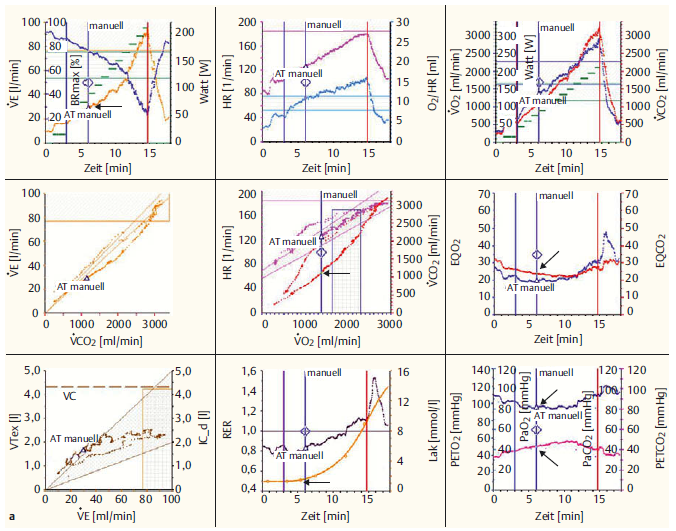
\includegraphics[width=135mm]{Bilder/9fieldcomplex.png}
	\caption[Beispielhafte 9-Felder-Grafik mit Markierungen für VT1]{Beispiel einer 9-Felder-Grafik einer jungen sportlichen Frau mit Markierungen für VT1~\cite{Kroidl.2015}}
	\label{pic:pic2}
\end{figure}
%
Anhand eines Pfeils und einer vertikalen Linie mit einer kleinen Raute wurde in den Feldern 1, 4, 5, 6, 8 und 9 die VT1 markiert. Die Plots enthalten noch weitere Cursor, die für andere diagnostische Anwendungen relevant sind. Die Felder enthalten sehr viele Informationen, weswegen die gesamte Grafik für einen Anwender ohne ausreichendes Hintergrundwissen sehr kompliziert aussehen wird. In Abb.~\ref{pic:pic3} ist die gleiche Grafik mit Markierungen für die VT2 zu sehen. Der Rest der Grafik unterscheidet sich nicht zu der in Abb. \ref{pic:pic2}. Die Plots lassen sich sehr gut zum Vergleich unterschiedlicher Felder und Auswertungsmethoden verwenden. Mit der 9-Felder-Grafik lassen sich Schwellenbestimmungen gut evaluieren und auf Übereinstimmung der Werte prüfen. Allerdings müssen die Graphen zuerst manuell ausgewertet werden. Sie sind für die Zwecke und Kunden von cardioscan zu komplex, da auch zu viele Plots für die Trainingsbereichsplanung wenig relevant sind. Es wird eine Darstellung benötigt, in der lediglich die bereits algorithmisch bestimmten ventilatorischen Schwellen eingefügt werden und die keine irrelevanten Informationen beinhaltet. Der Kunde soll ein Ergebnis generiert bekommen, welches nicht mehr händisch ausgewertet werden muss und einfacher nachvollziehbar ist.

\begin{figure}[H]
	\centering
	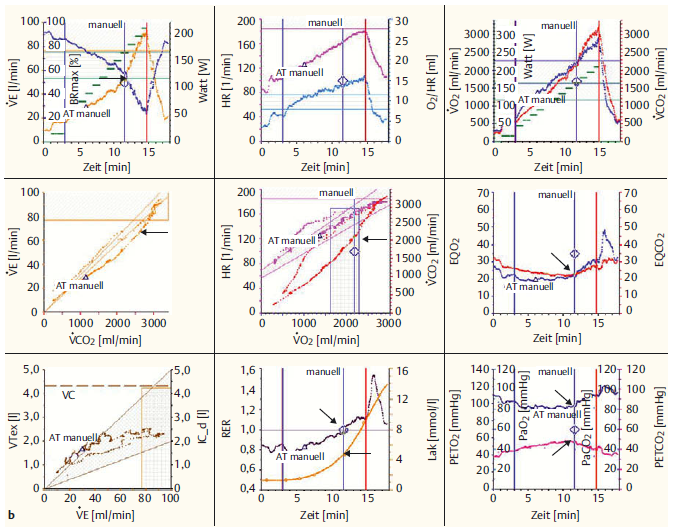
\includegraphics[width=135mm]{Bilder/9fieldplot.png}
	\caption[Beispielhafte 9-Felder-Grafik mit Markierungen für VT2]{Beispiel einer 9-Felder-Grafik einer jungen sportlichen Frau mit Markierungen für VT2~\cite{Kroidl.2015}}
	\label{pic:pic3}
\end{figure}
%
Zur Bestimmung von VT1 und VT2 existieren nun mehrere Möglichkeiten. Die wissenschaftlich am erfolgreichsten angewandten Methoden wurden 2012 offiziell zusammengefasst und auf vier je Schwelle reduziert~\cite{Westhoff.2012}. Da die Evaluation aller aufgeführten Methoden zeitlich zu umfangreich wäre, wird sich in dieser Arbeit nur auf die jeweils zwei renommiertesten Methoden konzentriert. Tab.~\ref{tab:tabelle2} listet diese gegenübergestellt für VT1 und VT2 auf und nennt die relevanten Messwerte sowie die entsprechenden Plots der 9-Felder-Grafik.

\begin{table}[H]
	\centering
	\caption{Ausgewählte Methoden zur Bestimmung von VT1 und VT2}
	\medskip
	\begin{tabularx}{\textwidth}{X X}
		\toprule
		\textbf{VT1} & \textbf{VT2} \\
		\midrule
		\midrule
		\begin{titemize}
			\item V-Slope-Methode: erster überproportionaler Anstieg von \acs{VCO2} gegenüber \acs{VO2} (Feld 5)
			\item Anstieg von \ac{EQO2} ohne gleichzeitigen Anstieg von \ac{EQCO2} (Feld 6)
		\end{titemize}
		&\begin{titemize}
			\item überproportionaler Anstieg von \acs{VE} gegenüber \acs{VCO2} (Feld 4)
			\item Anstieg von \ac{EQCO2} (Feld 6)
		\end{titemize}\\
		\bottomrule
	\end{tabularx}
	\label{tab:tabelle2}
\end{table}

\subsubsection{Bestimmung der VT1}

Die erste Methode zur Bestimmung der VT1 ist die Begutachtung des sogenannten "`V-Slopes"' in Feld 5 nach Beaver et al.~\cite{Beaver.1986}. Die Nomenklatur bezieht sich auf die beiden miteinander verglichenen Volumenströme (Flows) \acs{VCO2} und \acs{VO2} sowie die sich verändernde Steigung (engl. \textsl{slope}) des Graphen. Hierbei geht es um die Identifizierung charakteristischer Knickpunkte im \acs{VCO2}/\acs{VO2}-Verhältnis als Indikator für das Exzess-\acs{CO2}. Dieser grafische Vergleich der Volumenströme ist sehr stark vereinfacht und idealisiert als schematischer Beispielplot in Abb.~\ref{pic:pic4} zu sehen.

\begin{figure}[H]
	\centering
	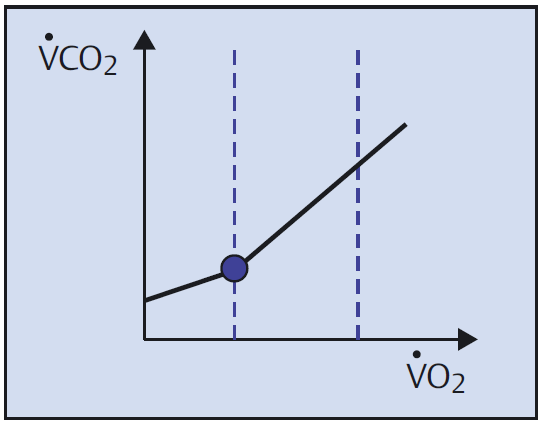
\includegraphics[width=50mm]{Bilder/vslope.png}
	\caption[Schematische Darstellung der V-Slope-Methode]{Schematische Darstellung der V-Slope-Methode, bei der \acs{VCO2} mit \acs{VO2} grafisch miteinander verglichen werden; VT1 ist die erste überproportionale \acs{VCO2}-Zunahme~\cite{Kroidl.2015}}
	\label{pic:pic4}
\end{figure}

Anhand der gestrichelten Linien sind VT1 (links) und VT2 (rechts) markiert. VT1 wird zusätzlich durch den blauen Punkt hervorgehoben. Bei VT1 ist erkennbar, dass \acs{VCO2} gegenüber \acs{VO2} durch das zusätzliche Exzess-\acs{CO2} aus der Laktatpufferung stärker ansteigt. Wo eine zweite deutliche Zunahme von \acs{VCO2} zur Kompensation der metabolischen Azidose erkennbar ist, kann ggf. je nach Qualität des Graphen auch VT2 gekennzeichnet werden, weshalb in der Abbildung durch die rechte gestrichelte Linie auch VT2 angedeutet ist. Dies wird allerdings lediglich für Vergleiche mit anderen Methoden getan und zählt nicht als gängige VT2-Methode.\\
Ebenfalls anwendbar ist die gleichzeitige Analyse der Atemäquivalente \acs{EQCO2} und \acs{EQO2} in Relation zur Zeit in \si{\minute} oder alternativ der Belastung (\acs{W} bzw. \acs{WL}) in \si{\watt} in Feld 6. Physikalisch werden diese durch das Verhältnis aus \acs{VE} und dem Flow des jeweiligen Gases definiert. 
%
\begin{flalign}
EQO_2 = \frac{\dot{V}E}{\dot{V}O_2}  &\hspace{2cm} EQCO_2 = \frac{\dot{V}E}{\dot{V}CO_2}
\label{eq:formel8}
\end{flalign}
%
Sie besitzen keine Einheit und beschreiben, wie viel geatmet werden muss, um einen Liter \acs{O2} aufzunehmen bzw. \acs{CO2} abzugeben. Der Tiefpunkt der \acs{EQO2}-Kurve wurde 1958 von Hollmann als Punkt des optimalen Wirkungsgrades (\acs{POW}) deklariert, welcher sich mit VT1 deckt~\cite{Kroidl.2015}. Dies ist auch in Abb.~\ref{pic:pic5} zu erkennen. Die Grafik zeigt ebenfalls vereinfacht ein Idealschema und die grafische Darstellung der \acs{EQO2}-Kurve. Auch hier sind anhand der gestrichelten Linien beide Schwellen (VT1 links, VT2 rechts) markiert. Danach beginnt die Laktatbildung und die Ventilation nimmt im Zuge der \acs{CO2}-Elimination zu, wodurch vorerst nur die \acs{EQO2}-Kurve beginnt, anzusteigen.

\begin{figure}[H]
	\centering
	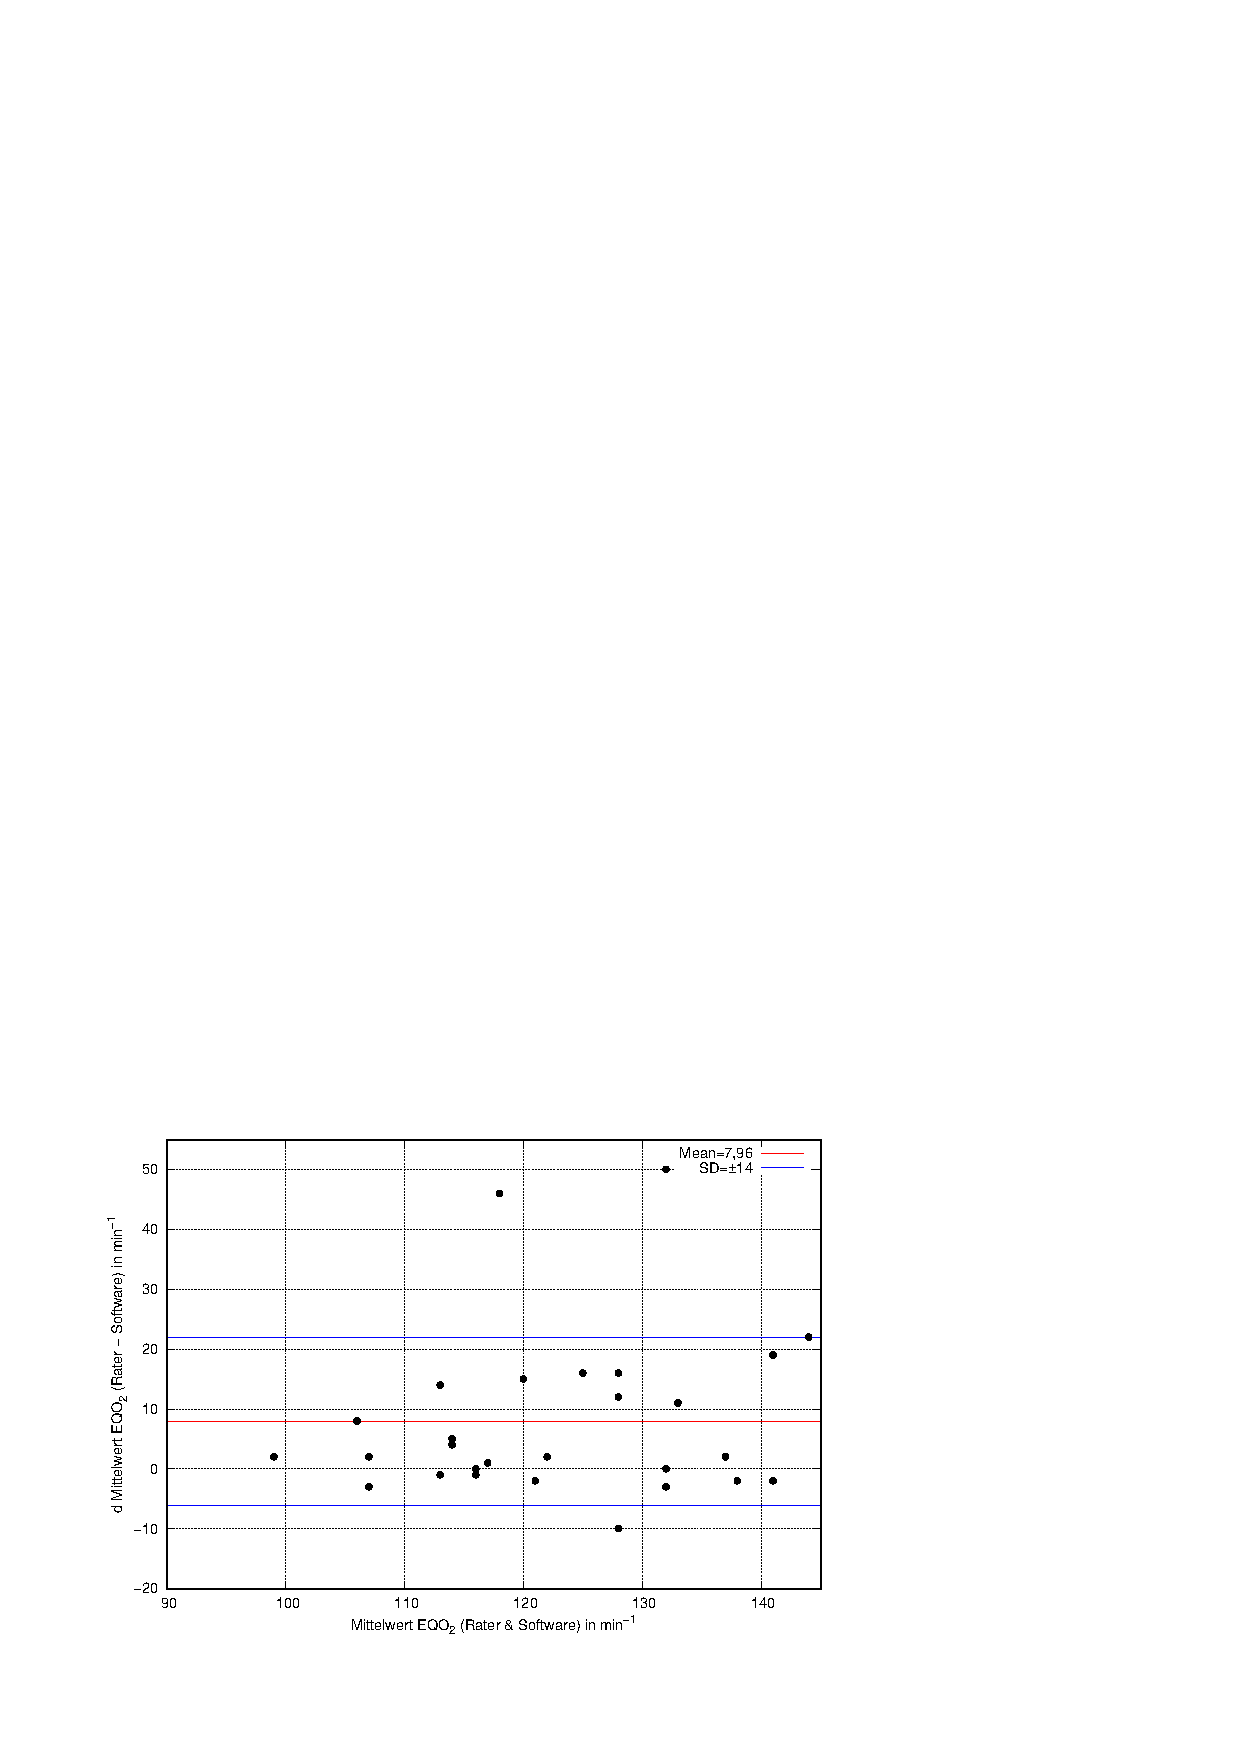
\includegraphics[width=50mm]{Bilder/eqo2.png}
	\caption[Schematische Darstellung des \acs{EQO2}]{Schematische Darstellung des \acs{EQO2} relativ zu der Zeit oder der Leistung \acs{WL}; VT1 ist der Tiefpunkt der Kurve~\cite{Kroidl.2015}}
	\label{pic:pic5}
\end{figure}

\subsubsection{Bestimmung der VT2}

Wie in Abb.~\ref{pic:pic5} durch die rechte gestrichelte Linie zu sehen, ist die VT2 ebenfalls in Feld 6 durch Betrachtung der Atemäquivalente bestimmbar. Dazu wird jedoch die \acs{EQCO2}-Kurve analysiert, wie schematisch in Abb.~\ref{pic:pic6} verdeutlicht. Diese nimmt für üblich eine charakteristische "`Badewannenform"' an~\cite{Kroidl.2015}.

\begin{figure}[H]
	\centering
	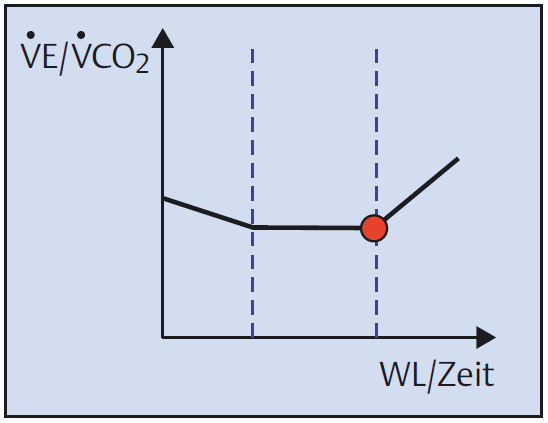
\includegraphics[width=50mm]{Bilder/eqco2.png}
	\caption[Schematische Darstellung des \acs{EQCO2}]{Schematische Darstellung des \acs{EQCO2} relativ zu der Zeit oder der Leistung \acs{WL}; VT2 ist der Anstieg von \acs{EQCO2}~\cite{Kroidl.2015}}
	\label{pic:pic6}
\end{figure}

VT2 wird durch die rechte Linie und den orangefarbenen Punkt markiert. Sie wird in dem Bereich gesetzt, an dem \acs{EQCO2} deutlich sichtbar ansteigt. Dort ist ebenfalls die Kompensation der metabolischen Azidose aufgrund des Ventilationsanstiegs, der sich auch in \acs{VCO2} widerspiegelt, erkennbar. Die Gegenüberstellung von \acs{VE} und \acs{VCO2} in Feld 4 wird jedoch als Goldstandard für die VT2-Bestimmung behandelt~\cite{ScharhagRosenberger.2013}. Dabei wird auf Erkenntnisse von Meyer et al. verwiesen, die mit dieser Methode bei einer Vielzahl an Probanden die VT2 (damals "`anaerobe Schwelle"') bestimmen konnten~\cite{Meyer.2005}.

\begin{figure}[H]
	\centering
	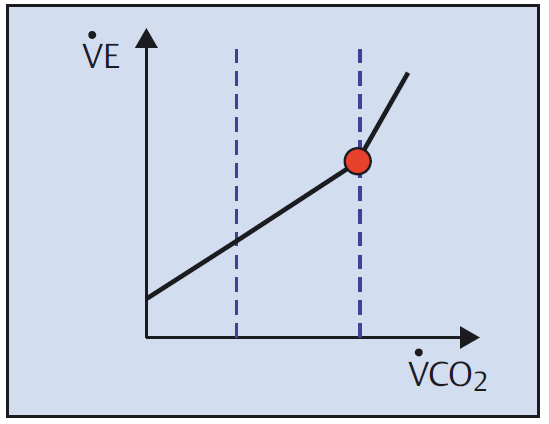
\includegraphics[width=50mm]{Bilder/field4.png}
	\caption[Schematische Darstellung von \acs{VE} relativ zu \acs{VCO2}]{Schematische Darstellung von \acs{VE} relativ zu \acs{VCO2}; VT2 ist der erste überproportionale Anstieg von \acs{VE}~\cite{Kroidl.2015}}
	\label{pic:pic7}
\end{figure}

In Abb.~\ref{pic:pic7} ist diese Methode vereinfacht visualisiert. Diese Grafik weist Analogien zum V-Slope auf, da auch zwei Volumenströme miteinander verglichen und auch hier die Schwellen mithilfe von Knickpunkten bestimmt werden. An der rechten gestrichelten Linie und dem orangen Punkt ist die zur Azidose-Kompensation einsetzende Hyperventilation bei ausgelastetem Bicarbonat-Puffer markiert~\cite{ScharhagRosenberger.2010} . Dies entspricht auch hier der Position von VT2.\\
Die V-Slope-Methode wird häufig als allgemeiner Goldstandard betitelt~\cite{ScharhagRosenberger.2013}. Dennoch wurde bereits von Friederike Scharhag-Rosenberger~\cite{ScharhagRosenberger.2010} und Wilfried Kindermann~\cite{Kindermann.2004} vom Institut für Sport- und Präventivmedizin Saarbrücken festgestellt wurde, dass ansteigende Intensitäten bei Stufentests für Artefakte sorgen können und deshalb stets differenziert ausgewertet werden müssen. Generell sollten unterschiedliche Methoden angewandt und zur Auswertung kombiniert werden, um Vergleiche innerhalb einer individuellen Diagnostik anstellen zu können~\cite{ScharhagRosenberger.2010}.
%\clearpage
\section{Problemstellung \& Ziele der Arbeit}

Die Bestimmung der ventilatorischen Schwellen in der Leistungsdiagnostik ist ein modernes und häufig empfohlenes Verfahren zur Trainingsplanung und daher für cardioscan ein sinnvolles Instrument. Momentan nutzt die Firma einen Algorithmus, der vom RQ abhängig ist. VT2 wird dort gesetzt, wo dieser den Wert eins erreicht. Begründet wird diese Verfahrensweise dadurch, dass Fettsäuren in körperlicher Ruhe den oxidativen Hauptenergielieferanten verkörpern, der RQ dann normalerweise bei ca. 0,7 liegt und mit zunehmender Belastung langsam ansteigt. Diefenthaeler et al.~\cite{Diefenthaeler.2017} und Zagatto et al.~\cite{Zagatto.2012} konnten dies in ihren Studien untermauern. Leti et al. hingegen machten die Beobachtung, dass die Belastungsintensität bei RQ = 1 deutlich von der objektiv mit VT2 assoziierten Intensität abwich~\cite{Leti.2012}. Dem sind besonders die Einflussfaktoren Trainingszustand sowie Belastungsart und -protokoll zugrundeliegend. Die Problematik wird zusätzlich durch den Fakt verstärkt, dass der Respiratorische Quotient (\acs{RQ}) auf unterschiedliche Weise, z.B. durch kohlenhydrathaltige Ernährung, akut beeinflussbar ist~\cite{ScharhagRosenberger.2010}. cardioscan arbeitet darüber hinaus mit Stufenprotokollen und nutzt hauptsächlich Fahrradergometer. Daraus können Abweichungen resultieren, wenn beispielsweise Laufathleten, die nicht häufig Fahrrad fahren, relativ frühzeitig muskulär ausbelastet sind, obwohl der RQ noch unterhalb von 1 liegt. Eine kardiorespiratorische Ausbelastung läge somit noch nicht vor und die VT2 wäre faktisch noch nicht erreicht~\cite{Tzvetkov.2008}. Zur Bestimmung der VT2 ist das Erreichen des Maximums jedoch unabdingbar~\cite{ScharhagRosenberger.2013}. Gemäß der Literaturempfehlungen wurden daher mehrere alternative Verfahren ausgewählt.\\
Zur Bestimmung der VT1:
%
\begin{itemize}
	\item V-Slope-Methode durch Analyse von \acs{VCO2} zu \acs{VO2}
	\item Äquivalent-Methode und alleiniger Anstieg von \acs{EQO2}
\end{itemize}
%
Zur Bestimmung der VT2:
%
\begin{itemize}
	\item Identifizierung des Anstiegs von \acs{VE} gegenüber \acs{VCO2}
	\item Äquivalent-Methode und Anstieg von \acs{EQCO2}
\end{itemize}
%
Als Referenz für VT2 wurde bei den Testmessungen die momentane Methode RQ = 1 angewandt.\\
Im Rahmen der Arbeit werden mithilfe der Messungen folgende Fragen behandelt:
%
\begin{enumerate}
	\item Eignet sich der metabolicscan zur Bestimmung ventilatorischer Schwellen?
	\item Mit welcher Methode können die Schwellen optimal bestimmt werden?
	\item Ist eine genauere Bestimmung der VT2 mit den neuen Methoden möglich?
\end{enumerate}
%
Ziel dieser Arbeit war die Durchführung von Testmessungen sowie Evaluierung der genannten Methoden mit dem metabolicscan. Hierfür bestimmten mehrere Instanzen unabhängig beide Schwellen. Deren Auswertungen wurden miteinander verglichen und die Korrelation der Ergebnisse analysiert.
\clearpage